\documentclass[../main/main.tex]{subfiles}

\newdate{date}{13}{11}{2020}

\begin{document}


\chapter{Introduction to metapopulation models}
\marginpar{ \textbf{Lecture 14.} \\  \displaydate{date}. \\ Compiled:  \today.}

\section{Spatial spread of epidemics}
Let us start now to dig deeper adding some complexity to our models. In particular now we want to understand why \textit{spatial spread} of epidemics is important, and its possible effect over public policies. It allows us to estimate the \textbf{invasion risk} for a given territory, hence understanding whether a place is more likely to develop an epidemic. In this way we are able to model and realize the \textbf{conditions for containment}, since containing an epidemic spatially helps in its management. Moreover, we will discuss about the so called \textbf{spatial coupling}, that is to say how the epidemic in a given area influences the epidemic in another. This should have explained us why \textbf{spatial information} is an \textbf{essential ingredient} in epidemiology: we need to know where the epidemic is at a given moment in order to take the proper countermeasures.

There might be different \textbf{drivers} of spatial transmission:
\begin{itemize}
    \item \textbf{direct} transmission among humans: the spatial spreading of epidemics is strongly affected by the \textit{human mobility}. Hence the pathogen spreads carried by travelling individuals;
    \item \textbf{vector borne}: the spatial propagation requires both \textit{human mobility} and the local presence of \textit{competent vector} (mosquitos, rats...). Mobility for vectors is also possible, too;
    \item \textbf{different drivers}, such as food borne, environmental diseases, zoonotic pathogens, etc.
\end{itemize}

As said, \textbf{human mobility}\footnote{Human mobility: Models and applications, Barbosa et al. Physics Reports 734 (2018)} behavior determines the spatiotemporal pattern of spreads. This should take into account that there exist \textbf{different types} of mobility, and the actual kind becomes relevant according to the epidemic and the epidemiological questions we are facing.

\subsection{Human mobility}
\label{section:human_mobility}

There are actually different types of data for the human mobility network. For instance, \textbf{air travelling} data is collected by the International Air Transport Association (IATA). It can be actually purchased, since the information publicly available is limited. There are two \textbf{types} of this data:
 \begin{itemize}
     \item \textbf{segment}: number of seats for each company between two airports;
     \item \textbf{origin-destination}: number of passengers travelling between origin-destination, obtained from the tickets purchased.
 \end{itemize}
Doing a similar analysis to the one we have done so far for the “air” network, one can note two facts related to the number of connections and the number of passengers: both \textbf{topology} and \textbf{traffic distribution} are \textbf{heterogeneous}.

\begin{figure}[h!]
\centering
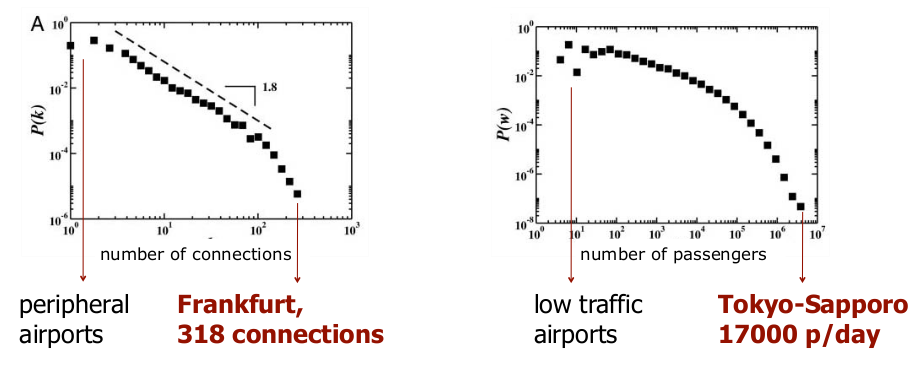
\includegraphics[width=1.0\textwidth]{../lessons/image/14/image01.png}
\caption{\label{fig:13_01} Whole segment network worldwide, 2002. Topology of the network and flux of passengers graphical analysis.}
\end{figure}

We can indeed find some \textbf{scaling relations} between fluxes, number of connections and population, as one can see from Fig. \ref{fig:13_02}. The average number of route $i \to j$ is determined by a non linear function of the traffic in airports, and it has form $w_{ij} \sim (k_i k_j)^\theta$ with $\theta =0.5$ and $N_i \sim k_i^{\phi}$ with $ 0.5\le \phi\le 1.5$, where $k_i$ is the traffic at the origin and $k_j$ at the destination. Values for $\theta$ and $\phi$ are computed empirically.

\begin{figure}[h!]
\centering
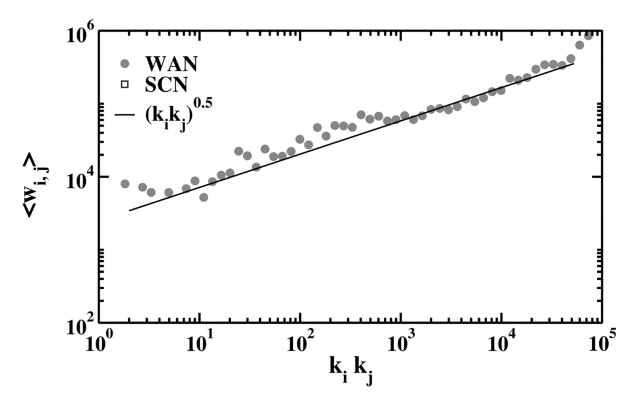
\includegraphics[width=0.5\textwidth]{../lessons/image/14/image02.png}
\caption{\label{fig:13_02} Whole segment network worldwide, 2002. Scaling relation.}
\end{figure}

Another type of mobility one may encounter is the so called \textbf{commuting}. This information is obtained from census of different countries and it mainly deals with locations of residence and work. For this reason, \textit{spatial resolution} is highly \textit{variable} and depends actually on the country: local/regional administrations can be actually organized differently within states. Moreover, we can make the aforementioned graphical analysis also for commuting network.

\begin{figure}[h!]
\centering
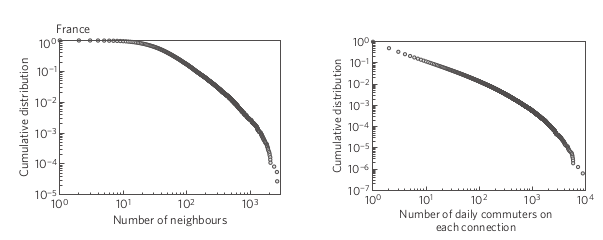
\includegraphics[width=0.8\textwidth]{../lessons/image/14/image03.png}
\caption{\label{fig:13_03}  Topology of the network and flux of passengers graphical analysis for commuting network.}
\end{figure}

We want now to point out the \textbf{differences} between the \textit{air travelling} and the \textit{commuting} networks. In order to do so, first we obviously need to use the same spatial resolution: this is why researchers defined \textbf{macro urban areas} centered around airports. Now we are able to look at what differs one network from the other. The first feature one may want to analyze is the average \textbf{daily number of travellers} in a certain area: it is about 1000 for the air travel, while 20'000 for the commuting network. Order or magnitudes are indeed different. Another important point is the \textbf{fraction of daily travellers}: it is defined as the probability to travel per time unit, namely the \textit{daily} flux of travellers normalized to the catchment population of an area assuming that all people have the same probability to travel. Empirically, we observe that is more probable to commute ($10^{-2} days^{-1}$) rather than air travel ($10^{-3} days^{-1}$). Finally, \textbf{time scales} for the two processes are different. One should first define what is a \textit{time scale}: we can refer to it as the \textit{length of the stay in the destination}, or more generically as the \textit{time elapsed from one trip to another}. This quantity when one travels by plane is usually of order days/weeks, whereas commuting is a matter of hours since at workplace we spend order of hours. In conclusion, \textbf{commuting} has a \textbf{faster dynamics} and leads to a \textbf{higher} level of \textbf{mixing}.

One another type of data that is available is the one shared privately by \textbf{telephone} providers. Information is recorded for each call and/or SMS: for instance time, caller ID, recipient ID, call duration and cellular tower. Using the position of the latter ones one may be able to reconstruct individual level trajectories. Obviously, for privacy, users are anonymized. Some \textbf{challenges} that may arise using this kind of data are the following: for \textbf{statistical reliability} the analysis is restricted to users that call \textit{more frequently}, but this actually can turn out to be not precise since many locations can still be missed. Another issue is that the area covered by the cell tower is highly variable: towers are more dense in densely populated area, whereas the \textbf{spatial resolution} is \textit{rural area} is very \textbf{poor}. This kind of data is really important and accurate: one can reconstruct individual trajectories and the mean of transport used and, eventually, why. For many low income countries this is actually the \textbf{main source of information} regarding mobility, despite it is available worldwide. Some drawbacks are that statistically this data must be treated carefully and poses statistical challenges, also from a numerical point of view. Moreover, data cannot be shared across groups for a matter of validation.

Other data can be collected from \textbf{GPS}, exploited by some apps or from research projects. This comes with the greatest level of accuracy on movement trajectories: \textbf{spatial resolution} is about few \textit{meters} and \textbf{temporal resolution} is about \textit{seconds}. However, devices with GPS are a really small subset ($10^3$) compared to $\sim 10^6$ mobile phones. Data can be collected by other \textbf{mobile application services} (e.g. Google, Twitter, Facebook...), it can give high spatial resolution, being it based on GPS, but the population may not be representative. Note that, because of some special events, data can be \textbf{donated}: Google, Apple have been sharing their data for good initiatives in helping against the fight or COVID19. An other \textbf{historical way} to collect migration was to trace the position of some US Federal banknotes \footnote{www.wheresgeorge.com}: their trajectories are likely a convolution of the mobility of several individuals. Finally, annual information of residence from individual tax return files in the US can describe \textbf{migration}, which has a time scale that spans over years.

As one may imagine \textbf{data} is very \textbf{heterogeneous}, being heterogeneous the sources where we collect it from. Heterogeneity can be seen in spatial resolution, individuals-level/origin-destination fluxes/seats, broken down per transportation media or per purpose of the trip. Since every dataset provides \textbf{partial information}, one may think to try to \textbf{combine} some of them. For instance, this cannot be done for air-travel and commuting network, being the spatial ranges very different. In addition, combining cell-phones data and commuting we are able to extract commuting proxies from cell-phone data. Finally, we should state that we cannot spot clearly the differences that occur for people of different ages: among air travellers indeed there are few children and old people, and statistically they look like the same and cannot be distinguished.



\subsection{Modelling Human Mobility}

Let us now discuss what models all the data collected so far can lead to. There are many types of model we can think of, starting from \textit{individuals-level} models or \textit{population-level} ones. As one can imagine, in the \textbf{individuals-level} models we model trajectories of individual using mathematical tools that might include stochasticity: random walk, brownian motion, Levy flight or preferential return, but there are actually many others.

Regarding instead \textbf{population level models} we try to model fluxes of individuals, therefore adding some layers of abstraction and generalization: we want to find for instance the \textit{Origin-Destination} matrices. There are two main families for these kind of models: \textbf{gravity models}, or \textbf{intervening opportunity models}.

The \textbf{Gravity Model} was first introduced by G.K. Zipf. He took inspiration from Newton's law of gravitation in order to describe \textbf{mobility flows}:
\begin{equation}
    T_{ij} \propto \frac{N_i N_j}{d_{ij}}
\end{equation}
where $N_i$ is the population in $i$-th site and $d_{ij}$ is the distance between nodes $i$ and $j$. The last formula can be written in a more general formula as it follows:
\begin{equation}
    T_{ij} = C M_i M_j F(d_{ij}), \qquad M_i = N_i^\alpha \quad M_j = N_j^\gamma
\end{equation}
where $F(d_{ij})$ is a general function that is either a power law of the kind $d_{ij}^\beta$ or exponential form $e^{-\beta d_{ij}}$ or a combination of both.
This model actually permits to fit very well the data, despite there are no general values for the fitting parameters: they do vary according to the spatial granularity. A possible workaround for this problem was to introduce the formula of \textit{Balcan et al PNAS 2009} ($T_{ij} = C \frac{N_i^\alpha N_j^\gamma}{e^{\beta d_{ij}}}$) which was fitted to 29 different countries spread across all continents.
The main \textbf{result} was that, when data is aggregated at the \textit{same level of spatial resolution}, the same parameters are able to model well the mobility fluxes in all countries.

\begin{figure}[h!]
\centering
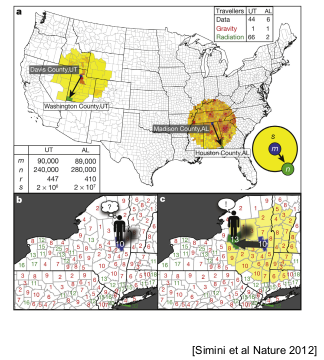
\includegraphics[width=0.4\textwidth]{../lessons/image/14/image04.png}
\caption{\label{fig:13_04} Graphical description for the radiation model. Individual is more likely to move where opportunities are more, since we use their number as a metric.}
\end{figure}

Another historical model for the mobility was the so called $\textbf{radiation model}$ (see Fig. \ref{fig:13_04}). It was introduced by Stouffer (1940). He noticed that the \textit{key} driver of migration was the number of \textbf{intervening opportunities} or the \textbf{cumulative number} of opportunities between the origin and the destination. However, definition of \textit{"opportunities"} was intentionally left vague and they assume a different meaning with respect to the system we are dealing with.


Resulting fluxes in this way are independent of $p(z)$ and are parameters free:
\begin{equation}
    T_{ij} = O_i \frac{1}{1-\frac{N_i}{M}}\frac{N_i N_j}{(N_i+S_{ij})(N_i+N_j+S_{ij})}
\end{equation}
where $S_{ij}$ is the population in the radius $d_{ij}$ and $M = \sum_i N_i$. The advantage that we do not need any parameters in order to use this model: it is useful in epidemiology when the only information we have is the population distribution (it usually happens for low developed countries). However, the goodness of fit depends on the spatial resolution.



\section{Integrating Human Mobility in Epidemic Models}

Now we want to use the knowledge we have acquired so far to describe better how Human Mobility affects epidemic spreading. In order to do it, we will borrow from ecology the concept of \textbf{metapopulation models}. The last was introduced to study the interplay between stochasticity and spatial heterogeneities\footnote{Levins Bull. Entomol. Soc. Am., 15 (3) (1969).}: the entire population was divided in \textbf{patches} which are discrete entities (see \ref{fig:13_05}). It follows that there may be two different levels of mixing: \textit{local}, that occurs within a patch, or \textit{global} that occurs among patches. It is a \textbf{coarse grained} description, and patches can be seen as the new elementary units for our network.

\begin{figure}[h!]
\centering
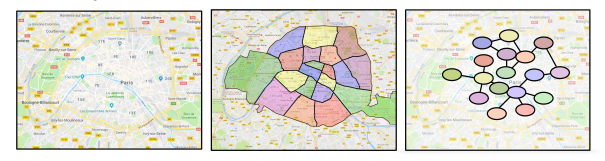
\includegraphics[width=1\textwidth]{../lessons/image/14/image05.png}
\caption{\label{fig:13_05} Population is divided in discrete entities, the so called \textit{patches} that will become our new elementary units when dealing with network.}
\end{figure}

In ecology the dynamics is therefore driven by stochastic effects, which may lead for instance to extinction or recolonisation. This, obviously, will suggest us to find an analogy when dealing with epidemic models. However, one should keep into account that the \textbf{discrete nature of individual} is one of the most essential ingredients to describe the dynamics: it is meaningless to state that half an individual travels between two patches. The first models assumed that the mixing between patches occurred homogeneously, while more recently more complexity has been added: \textbf{mixing} among patches has started to be \textbf{mediated} by the \textbf{human mobility network} hence coupling the metapopulation perspective with network theory.


\subsection{SIR metapopulation model}

Let us discuss now how we can introduce the metapopulation concept into a model we have studied so many times: the \textit{SIR} model (see fig. \ref{fig:13_06}). The only difference here is that it is \textbf{not} an \textbf{individual-based} model any more. now we do not keep track of every indivudal, but we just monitor the occupation number of patches and compartments.

\begin{figure}[h!]
\centering
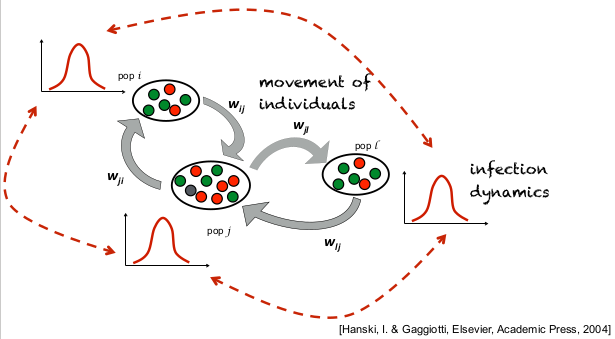
\includegraphics[width=0.7\textwidth]{../lessons/image/14/image06.png}
\caption{\label{fig:13_06} How we can model mobility and transmission dynamics using SIR metapopulation model}
\end{figure}

For each $i$-th patch we can define the following variables, as we did for the entire population before: $S_i(t)$, $I_i(t)$, $R_i(t)$, and obviously it holds that $N_i(t) = S_i(t) + I_i(t) + R_i(t)$ with clear meanings for each of them. Note that, given a total number of $V$ patches, it follows the definition of global variables:
\begin{subequations}
\begin{align}
    S(t) &= S_1(t) + S_2(t) + S_3(t) + ... + S_V(t) = \sum_i S_i(t) \\
    I(t) &= I_1(t) + I_2(t) + I_3(t) + ... + I_V(t) = \sum_i I_i(t) \\
    R(t) &= R_1(t) + R_2(t) + R_3(t) + ... + R_V(t) = \sum_i R_i(t) \\
    N(t) &= N_1(t) + N_2(t) + N_3(t) + ... + N_V(t) = \sum_i N_i(t)
\end{align}
\end{subequations}

The set of equations related to $i$-th node and the compartments is the following:
\begin{subequations}
\begin{align}
    \dv{S_i}{t}  &= -\beta \frac{I_i(t)S_i(t)}{N_i} + \mathcolorbox{yellow!40}{\Omega_i^S}\\
    \dv{I_i}{t} &= \beta \frac{I_i(t)S_i(t)}{N_i}  - \mu I_i(t) + \mathcolorbox{yellow!40}{\Omega_i^I}\\
    \dv{R_i}{t} &= \mu I_i (t) + \mathcolorbox{yellow!40}{\Omega_i^R}
\end{align}
\end{subequations}
where we have introduced $\Omega_i^X$ that is a measure of the \textit{in-flow} or \textit{out-flow} of people in compartment $X$. Note as the set of equations really resembles the SIR model we previously studied.

\marginpar{
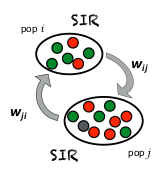
\includegraphics[width=\marginparwidth]{../lessons/image/14/image07.png}
\captionof{figure}{\label{fig:13_07} Mobility between two different patches occurs with probability $p_{ij} = w_{ij}/N_i$.}
}

We will now discuss how to compute $\Omega_i^X$ for which we need to model human mobility. The first assumption we make is that the mobility is a \textbf{Markovian process}. Indeed, this is the easiest model one can think of. We need now to model human mobility, and this can be done in the following way: we now that $N_i$ people live in $i$-th patch, and $w_{ij}$ is the number of people that travel $i \to j$. Therefore, the \textbf{probability} for an individual in $i$ \textbf{to travel} from $i$ to $j$ is:
\begin{equation}
    p_{ij} = \frac{w_{ij}}{N_i}
\end{equation}
The simplest possible model is when $p_{ij}$ is the same for all individuals \textbf{regardless} their \textit{infectious status} (S,I,R) and their \textit{travel history}. This is the Markovian assumption we stated above. As soon as an individual enters into a new population, she mixes completely within it and cannot be distinguished from other individuals any more. Moreover, she will be considered as part of that population from now on.

Travelling is a \textbf{binomial process}. The average number of individuals in compartment $X$ in $i$ travelling from $i$ to $j$ at each $t$ is:
\begin{equation}
   \expval{T_{ij}^X} = p_{ij} X_i(t) = \frac{w_{ij}}{N_i} X_i(t)
\end{equation}
Therefore, a formula for $\Omega_i^X$ can be the following:
\begin{equation}
    \Omega_i^X = \sum_j \left(\frac{w_{ji}}{N_j} X_j - \frac{w_{ij}}{N_i} X_i  \right)
\end{equation}
where, for the flux, we consider all the people that are entering patch $i$ from all possible other patches $j$, as well as all individuals exiting the node $i$ being their destination any other patch $j$.

We now recall the \textbf{assumptions} we have done so far. We have modelled mobility as a \textbf{Markovian process}. In other words, we assume that travellers mix with the population at destination and forget about travel origin. The implications hence are:
\begin{itemize}
    \item \textbf{travel trajectory} is \textit{random}: patch $i \to$ patch $j \to $ patch $l \to $ ...;
    \item we do \textit{not} take into account the \textbf{residence location};
    \item we do \textit{not} take into account the \textit{length of stay} while travelling.
\end{itemize}
At the end of the day we are modelling a \textbf{migration process}.
The Markovian assumption for mobility actually works well as long as \textbf{travels} are \textbf{not frequent}, that is to say that travelling rate is \textit{negligible} wrt epidemic time scales ($p_{ij} \ll \mu$). Moreover one should choose the Markovian assumption when we want to model the \textbf{short term dynamics} of an epidemic. In the real world, some situations where this hold at a first approximation are for instance:
\begin{itemize}
    \item air-travel and acute infections: for example flu or COVID 19. We have seen that travelling rate is about $10^{-3} days^{-1}$ that way smaller that their recovery rate $10^{-1} days^{-1}$;
    \item the early spread of COVID-19 or a flu pandemic. However, it does not work when we want to model the spreading in the long run (i.e. for large times).
\end{itemize}


\end{document}
